\documentclass[journal,12pt,twocolumn]{IEEEtran}

\usepackage{setspace}
\usepackage{gensymb}
\singlespacing
\usepackage[cmex10]{amsmath}

\usepackage{amsthm}

\usepackage{mathrsfs}
\usepackage{txfonts}
\usepackage{stfloats}
\usepackage{bm}
\usepackage{cite}
\usepackage{cases}
\usepackage{subfig}
\usepackage{graphicx}
\usepackage{longtable}
\usepackage{multirow}

\usepackage{enumitem}
\usepackage{mathtools}
\usepackage{steinmetz}
\usepackage{tikz}
\usepackage{circuitikz}
\usepackage{verbatim}
\usepackage{tfrupee}
\usepackage[breaklinks=true]{hyperref}
\usepackage{graphicx}
\usepackage{tkz-euclide}

\usetikzlibrary{calc,math}
\usepackage{listings}
    \usepackage{color}                                            %%
    \usepackage{array}                                            %%
    \usepackage{longtable}                                        %%
    \usepackage{calc}                                             %%
    \usepackage{multirow}                                         %%
    \usepackage{hhline}                                           %%
    \usepackage{ifthen}                                           %%
    \usepackage{lscape}     
\usepackage{multicol}
\usepackage{chngcntr}

\DeclareMathOperator*{\Res}{Res}

\renewcommand\thesection{\arabic{section}}
\renewcommand\thesubsection{\thesection.\arabic{subsection}}
\renewcommand\thesubsubsection{\thesubsection.\arabic{subsubsection}}

\renewcommand\thesectiondis{\arabic{section}}
\renewcommand\thesubsectiondis{\thesectiondis.\arabic{subsection}}
\renewcommand\thesubsubsectiondis{\thesubsectiondis.\arabic{subsubsection}}


\hyphenation{op-tical net-works semi-conduc-tor}
\def\inputGnumericTable{}                                 %%

\lstset{
%language=C,
frame=single, 
breaklines=true,
columns=fullflexible
}
\begin{document}
\newtheorem{lemma}{Lemma}[section]
\newcommand{\BEQA}{\begin{eqnarray}}
\newcommand{\EEQA}{\end{eqnarray}}
\newcommand{\define}{\stackrel{\triangle}{=}}
\bibliographystyle{IEEEtran}
\raggedbottom
\setlength{\parindent}{0pt}
\providecommand{\mbf}{\mathbf}
\providecommand{\pr}[1]{\ensuremath{\Pr\left(#1\right)}}
\providecommand{\qfunc}[1]{\ensuremath{Q\left(#1\right)}}
\providecommand{\sbrak}[1]{\ensuremath{{}\left[#1\right]}}
\providecommand{\lsbrak}[1]{\ensuremath{{}\left[#1\right.}}
\providecommand{\rsbrak}[1]{\ensuremath{{}\left.#1\right]}}
\providecommand{\brak}[1]{\ensuremath{\left(#1\right)}}
\providecommand{\lbrak}[1]{\ensuremath{\left(#1\right.}}
\providecommand{\rbrak}[1]{\ensuremath{\left.#1\right)}}
\providecommand{\cbrak}[1]{\ensuremath{\left\{#1\right\}}}
\providecommand{\lcbrak}[1]{\ensuremath{\left\{#1\right.}}
\providecommand{\rcbrak}[1]{\ensuremath{\left.#1\right\}}}
\theoremstyle{remark}
\newtheorem{rem}{Remark}
\newcommand{\sgn}{\mathop{\mathrm{sgn}}}
\providecommand{\abs}[1]{\vert#1\vert}
\providecommand{\res}[1]{\Res\displaylimits_{#1}} 
\providecommand{\norm}[1]{\lVert#1\rVert}
\providecommand{\sinc}{sinc}
%\providecommand{\norm}[1]{\lVert#1\rVert}
\providecommand{\mtx}[1]{\mathbf{#1}}
\providecommand{\mean}[1]{E[ #1 ]}
\providecommand{\fourier}{\overset{\mathcal{F}}{ \rightleftharpoons}}
%\providecommand{\hilbert}{\overset{\mathcal{H}}{ \rightleftharpoons}}
\providecommand{\system}{\overset{\mathcal{H}}{ \longleftrightarrow}}
	%\newcommand{\solution}[2]{\textbf{Solution:}{#1}}
\newcommand{\solution}{\noindent \textbf{Solution: }}
\newcommand{\cosec}{\,\text{cosec}\,}
\providecommand{\dec}[2]{\ensuremath{\overset{#1}{\underset{#2}{\gtrless}}}}
\newcommand{\myvec}[1]{\ensuremath{\begin{pmatrix}#1\end{pmatrix}}}
\newcommand{\mydet}[1]{\ensuremath{\begin{vmatrix}#1\end{vmatrix}}}
\numberwithin{equation}{subsection}
\makeatletter
\@addtoreset{figure}{problem}
\makeatother
\let\StandardTheFigure\thefigure
\let\vec\mathbf
\renewcommand{\thefigure}{\theproblem}
\def\putbox#1#2#3{\makebox[0in][l]{\makebox[#1][l]{}\raisebox{\baselineskip}[0in][0in]{\raisebox{#2}[0in][0in]{#3}}}}
     \def\rightbox#1{\makebox[0in][r]{#1}}
     \def\centbox#1{\makebox[0in]{#1}}
     \def\topbox#1{\raisebox{-\baselineskip}[0in][0in]{#1}}
     \def\midbox#1{\raisebox{-0.5\baselineskip}[0in][0in]{#1}}
\vspace{3cm}
\title{EE3900 Quiz2}
\author{W Vaishnavi\\AI20BTECH11025}
\maketitle
\newpage
\bigskip
\renewcommand{\thefigure}{\theenumi}
\renewcommand{\thetable}{\theenumi}
Download all latex-tikz codes from 
%
\begin{lstlisting}
https://github.com/vaishnavi-w/EE3900/blob/main/Quiz2
\end{lstlisting}
\section{3.18 a}
A causal LTI system has the system function 
\begin{align}
    H\brak{z} = \frac{1+2z^{-1}+z^{-2}}{\brak{1+\frac{1}{2}z^{-1}}\brak{1-z^{-1}}}
\end{align}
Find the impulse response of the system, $h[n]$
\section{Solution}
\begin{align}
    H\brak{z} &= \frac{1+2z^{-1}+z^{-2}}{\brak{1+\frac{1}{2}z^{-1}}\brak{1-z^{-1}}}\\
    &= \frac{2\brak{z^2 + 2z + 1}}{\brak{2z+1}\brak{z-1}}\\
    &= \frac{2\brak{3z+4/3}}{2z+1} -\frac{2\brak{z-7/3}}{z-1}\\
    &= H_1\brak{z}+H_2\brak{z}+H_3\brak{z}+H_4\brak{z}
\end{align}
where
\begin{align}
    H_1\brak{z} &= \frac{6z}{2z+1} = 3\brak{\frac{1}{1-\brak{-2z}^{-1}}},ROC_1 = |z|>\frac{1}{2}\\
    H_2\brak{z} &= \frac{-2z}{z-1} = -2\brak{\frac{1}{1-z^{-1}}},ROC_2 = |z|>1 \\
    H_3\brak{z} &= \frac{8}{6z+3} = \frac{4}{3}\brak{\frac{z^{-1}}{1-\brak{-2z}^{-1}}}ROC_3 = |z|>\frac{1}{2}\backslash \{0\} \\
    H_4\brak{z} &= \frac{14}{3z-3} = \frac{14}{3}\brak{\frac{z^{-1}}{1-z^{-1}}},ROC_4 = |z|>1 \backslash \{0\} 
\end{align}
Thus, ROC of $H(z) = |z|>\frac{1}{2}\backslash \{0\}$

The $\mathcal{Z}$ transform of a sequence of the form $a^nu[n]$ is given as,
\begin{align}
    \mathcal{Z}\brak{a^nu[n]} = \sum_{n=-\infty}^{\infty} a^nu[n]z^{-n} = \frac{1}{1-az^{-1}}\\
    a^nu[n] \xleftrightarrow{\text{\mathcal{Z}}} \frac{1}{1-az^{-1}}
\end{align}
with ROC $|az^{-1}|<1$

For a discrete signal $x[n]$ and it's $\mathcal{Z}$ transform $X(z)$ from time shifting property, we have
\begin{align}
    x[n] \xleftrightarrow{\text{\mathcal{Z}}} X(z)\\
    x[n-n_0] \xleftrightarrow{\text{\mathcal{Z}}} z^{-n_0}X(z)
\end{align}
That gives,
\begin{align}
    a^{n-n_0}u[n-n_0] \xleftrightarrow{\text{\mathcal{Z}}} \frac{z^{-n_0}}{1-az^{-1}}
\end{align}
with ROC for $n_0>0, |az^{-1}|<1$ except $z=0$

Taking the inverse $\mathcal{Z}$ transforms,
\begin{align}
    h_1[n] &= \mathcal{Z}^{-1}\brak{H_1\brak{z}} = 3\brak{-2^{-1}}^{n}u[n]\\
    h_2[n] &= \mathcal{Z}^{-1}\brak{H_2\brak{z}} = -2u[n]\\
    h_3[n] &= \mathcal{Z}^{-1}\brak{H_3\brak{z}} = \frac{4\brak{-2^{-1}}^{n-1}u[n-1]}{3}\\
    h_4[n] &= \mathcal{Z}^{-1}\brak{H_4\brak{z}} = \frac{14}{3}u[n-1]
\end{align}
Impulse response of the system
\begin{multline}
    h[n] = h_1[n]+ h_1[n] + h_1[n] + h_1[n] \\= u[n]\brak{3\brak{-2^{-1}}^n-2} + \frac{u[n-1]}{3}\brak{4\brak{-2^{-1}}^{n-1} + 14}
\end{multline}
\begin{figure}[h]
    \centering
    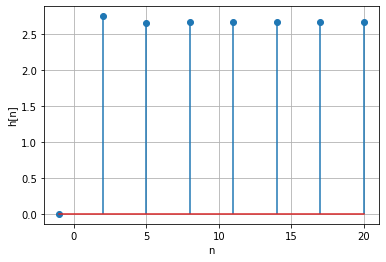
\includegraphics[width=\columnwidth]{signal.png}
    \caption{Plot of impulse response $h\brak{n}$}
    \label{fig:figure2}
\end{figure}
\end{document}
